\chapter{Tinjauan Pustaka dan Dasar Teori}

\section{Tinjauan Pustaka}

Berisi tugas akhir-tugas akhir terdahulu yang terkait dengan judul skripsi yang dilakukan. Hal ini meliputi skripsi atau tesis terdahulu yang terkait dengan judul skripsi yang diusulkan. Lakukan penguraian secara sistemastis dengan menjelaskan masalah apa yang dilakukan oleh tugas akhir terdahulu, kontribusi yang dilakukan, serta analisis penulis terkait dengan keunggulan dan keterbatasan tugas akhir. 

Setelah membahas berbagai tugas akhir terdahulu, maka alangkah baiknya penulis melakukan rangkuman terutama terkait dengan peluang pengeksplorasian atau tugas akhir yang akan dilakukan.


\section{Dasar Teori}

\subsection{\textit{Shell} Sistem Operasi}

\subsection{Linux, "\textit{Unix-like}", dan Standar POSIX}

\subsection{Beragam Usaha Pemberian Kompatibilitas Linux di Sistem Operasi Windows}

% Windows Subsystem for Linux bukan merupakan usaha pertama Microsoft ataupun satu-satunya solusi yang ada, baik oleh Microsoft maupun oleh pengembang pihak ketiga, dalam pengimplementasian kompatibilitas Linux atau \textit{Unix-like} di lingkungan sistem operasi Windows. Dalam sejarah, terdapat.

Windows Subsystem for Linux bukan merupakan satu-satunya cara yang pernah ada yang membawa kompatibilitas Linux atau Unix-like ke dalam lingkungan sistem operasi Windows. Dalam sejarah, terdapat berbagai solusi yang ditawarkan baik oleh Microsoft (sebelum WSL) maupun oleh pengembang pihak ketiga yang dapat digunakan pengguna untuk menambahkan kompatibilitas Linux/Unix-like ke perangkat komputer Windows mereka dengan popularitas yang beragam.

\subsubsection{Solusi Pihak Pertama (\textit{First Party}) oleh Microsoft}

Sebelum mengembangkan WSL, Microsoft memiliki sejumlah usaha terdahulu yang bertujuan membawa dukungan Linux/Unix-like ke dalam sistem operasi Windows. Dalam proses pengembangan Windows NT yang saat ini mendasari versi-versi Windows modern (Windows 2000 dan setelahnya), Microsoft mendesain sistem operasi tersebut sedemikian rupa agar bersifat modular dan mendukung berbagai macam "subsistem". Pada awal pengembangannya, Windows NT direncanakan memiliki tiga buah subsistem, yakni subsistem Win32, subsistem OS/2 (untuk mendukung interoperabilitas dengan sistem operasi OS/2 milik IBM), dan subsistem POSIX (untuk mendukung interoperabilitas dengan sistem-sistem berbasis Linux, UNIX, atau Unix-like yang sedang populer di kalangan bisnis pada masa itu). Seiring waktu, Microsoft memutus dukungan dan pengembangan lebih lanjut terhadap subsistem OS/2 karena adanya permasalahan bisnis dengan IBM.

Berbeda dengan subsistem OS/2 yang telah mati, dukungan dan pengembangan terhadap subsistem POSIX masih terus berjalan. Secara umum, terdapat tiga iterasi teknologi subsistem POSIX/UNIX yang dikembangkan oleh Microsoft:

\begin{enumerate}
    \item \textbf{Microsoft POSIX Subsystem.} Teknologi ini merupakan teknologi asli kembangan Microsoft yang ada sejak awal pengembangan Windows NT. Teknologi ini tersedia untuk sistem operasi Windows NT 3.1 hingga Windows 2000.
    \item \textbf{Windows Services for Unix (SFU).} Produk ini sesungguhnya adalah teknologi milik perusahaan bernama PTS yang dilisensikan kepada Microsoft. Produk ini menggantikan Microsoft POSIX Subsystem sejak sistem operasi Windows XP dan Windows Server 2003.
    %Teknologi yang membawahi (...) ini sejatinya merupakan hasil pengembangan
    \item \textbf{Subsystem for Unix-based Applications (SUA).}
    % Teknologi ini sejatinya merupakan pengembangan lebih lanjut dari SFU.
    % Teknologi ini pada awalnya bernama subsistem Interix dan berganti nama setelah Microsoft mengakuisisi perusahaan pengembangnya. Setelah akuisisi, produk ini tidak lagi berdiri sebagai produk terpisah, tetapi menjadi salah satu komponen dari Windows Services for Unix (SFU). Komponen ini tersedia sejak 
\end{enumerate}

% hingga sistem operasi Windows 7 meskipun dengan nama dan implementasi yang telah berganti dan popularitas yang semakin meredup. Meskipun Microsoft telah memiliki implementasi tersebut

% Reason against elaborationg further: The lack of new sources due to the nature of this topic that is "historical information".

%%% Usaha pencapaian kompatibilitas Linux atau \textit{Unix-like} di sistem operasi Windows umumnya dapat dikategorikan menjadi dua: usaha secara pihak pertama (\textit{first party}) oleh Microsoft dan usaha yang dilakukan oleh pihak ketiga (\textit{third party}) melalui perangkat lunak tambahan.

%%% \subsubsection{Usaha secara Pihak Pertama (\textit{first party}) oleh Microsoft}

%%% Windows Subsystem for Linux bukan merupakan usaha pertama Microsoft dalam meraih kompatibilitas dengan ekosistem POSIX. Dalam sejarah, Microsoft telah mencoba berbagai pendekatan dalam menanamkan implementasi subsistem UNIX di dalam Windows, baik secara sebagian maupun secara menyeluruh.
% https://link.springer.com/chapter/10.1007/978-1-4842-6038-8_1

\subsubsection{Solusi Pihak Ketiga (\textit{Third Party})}

Lorem ipsum

\begin{enumerate}
    \item \textbf{Colinux.}

    \item \textbf{Cygwin.}
\end{enumerate}

\subsection{Windows Subsystem for Linux}

Windows Subsystem for Linux merupakan usaha terbaru Microsoft dalam membawa kompatibilitas Unix/Linux ke dalam lingkungan Windows.

\subsection{Teknologi Penampilan Antarmuka Grafis dan Sistem Perjendelaan (\textit{Windowing System}) pada Lingkungan Linux: X11/Xorg dan Wayland}

\subsection{Dukungan Antarmuka Grafis pada Windows Subsystem for Linux: Windows Subsystem for Linux GUI (WSLg)}

Microsoft pertama kali menyatakan dukungan penjalanan perangkat lunak berantarmuka grafis (GUI) di Windows Subsystem for Linux versi 2 (WSL2) secara bawaan (\textit{built-in}) pada perhelatan pengembang tahunan Microsoft Build 2021.

Dalam pengembangan fungsionalitas antarmuka grafis pada Windows Subsystem for Linux, Microsoft berkomitmen untuk mengikuti standar yang telah ada pada lingkungan Linux.

\begin{figure}
    \centering
    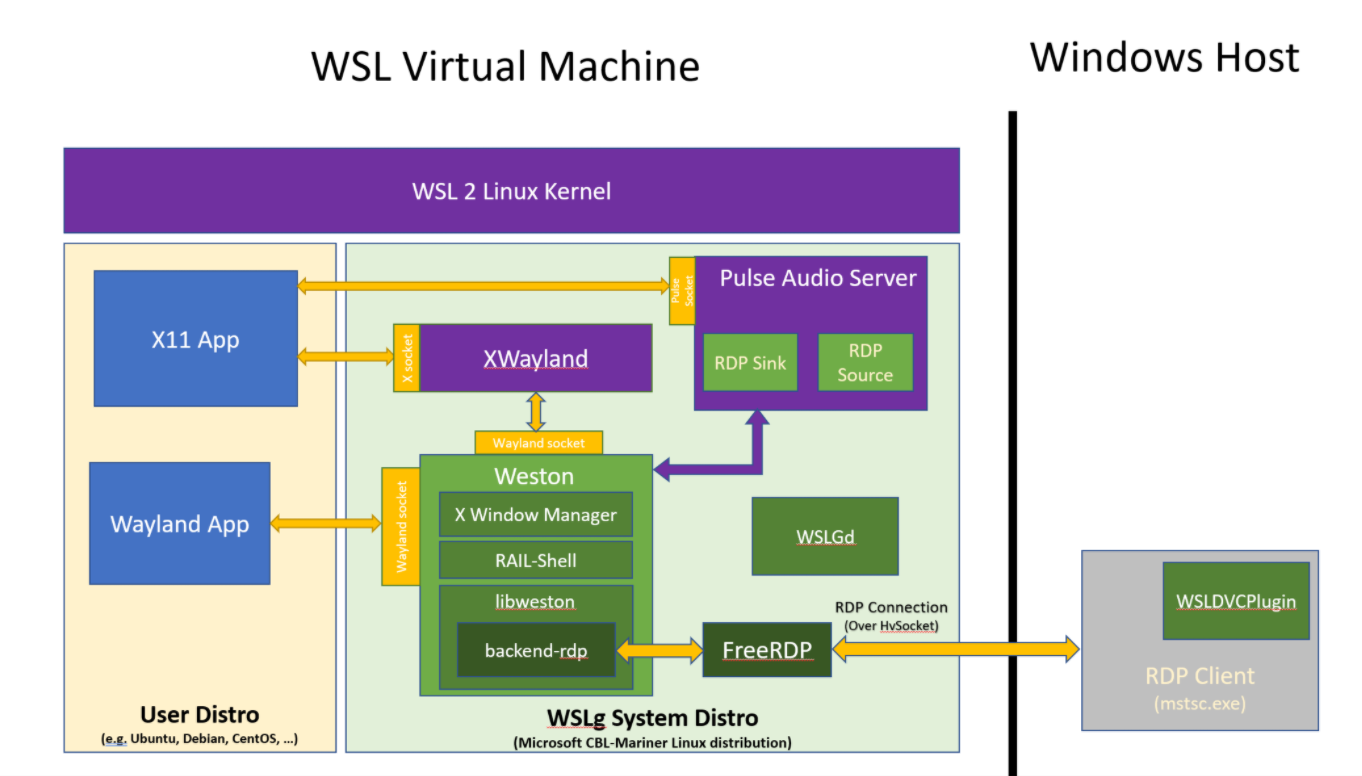
\includegraphics[width=0.5\linewidth]{wslg-architecture.png}
    \caption{Arsitektur Windows Subsystem for Linux GUI (WSLg)}
    \label{fig:enter-label}
\end{figure}

% https://link.springer.com/chapter/10.1007/978-1-4842-6873-5_1
% https://devblogs.microsoft.com/commandline/wslg-architecture/

\subsection{D-Bus}

\subsection{Windows App SDK}

\section{Analisis Perbandingan Metode}

Di dalam tinjauan pustaka hasil akhirnya adalah analisis secara kualitatif atau pun secara kuantitatif kelebihan dan kekurangan metode jika dikaitkan dengan masalah, batasan-batasan masalah dan solusi yang dinginkan. Analisis kuantitatif tidak wajib teapi mempunyai nilai tambah di dalam tugas akhir saudara. Bagian ini menjelaskan kenapa metode tersebut dipilih dan uraikan dengan lebih jelas metode pelaksanaan tugas akhir yang ingin Anda lakukan. 

\section{Pertanyaan Tugas Akhir (Jika Perlu)}

Pertanyaan tugas akhir bersifat opsional dan dapat ditambahkan untuk menekankan hal-hal yang hendak diketahui dari tugas akhir berdasar pada tujuan tugas akhir. Pertanyaan tugas akhir dikenal dengan RQ (\textit{Research Question}) dan harus memiliki keterkaitan dengan RO (\textit{Research Objective}). Satu RO dapat memiliki satu atau lebih dari satu RQ. 

